% !TEX root = ccsn.tex
\section{Detection sensitivity with Advanced gravitational wave detectors}
\label{sec:results}

To estimate how accurately we can infer the time evolution of $r=M_{\rm PNS}/R_{\rm PNS}^2$ in the
gravitational wave detector data, we have added \pcd{the} GW signal \pcd{from {\texttt s20S}} to 
100 Gaussian noise realisations whose power spectral density follows \pcd{the} advanced LIGO (aLIGO)
spectrum~\cite{aLIGOsens:2018} shown on Figure~\ref{fig:spectrum}. 

\begin{figure}
 \centering
 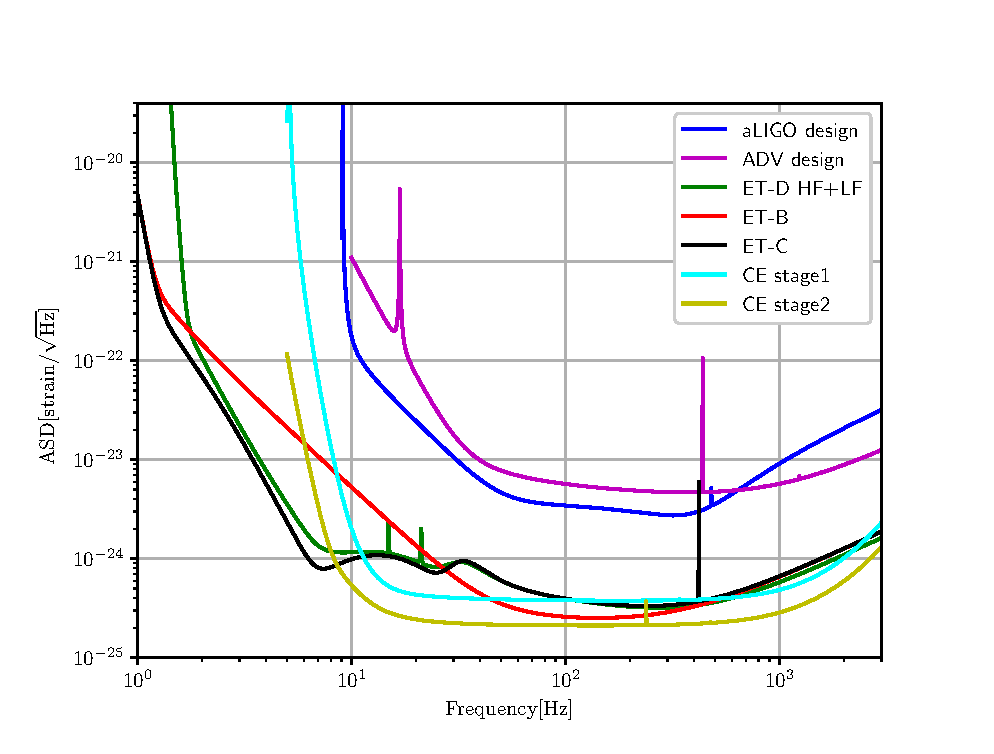
\includegraphics[width=0.5\textwidth]{plots/spectrum}
 \caption{Amplitude spectral density of the GW detectors advanced LIGO (aLIGO) and Advanced Virgo (ADV) at design sensitivity and of the proposed third generation detectors Cosmic Explorer and Einstein Telescope. Eintein Telescope sensitivity curve ET-B is obtained pushing second generation detector technology at its limit. ET-C and ET-D sensitivity curves correspond to a detector configuration where a low-power cryogenic low-frequency interferometer and a high-power room temperature high-frequency interferometer are sharing the same infrastructure~\cite{Hild_20211}. Cosmic Explorer design sensitivity will be achieved in two stages. Stage 1 (CE1) is expected to use the technology developed for the “A+” upgrade to advanced LIGO but scaled up to a 40 km detector while stage 2 (CE2) will implement state-of-the-art technology to decrease quantum and thermal noises~\cite{reitze2019cosmic}. } \label{fig:spectrum}
\end{figure}

We have varied the distance to the source, covering a large
range of distances for which a detection in second generation of gravitational wave detectors
is feasible. The source is optimally oriented with
respect to the gravitational wave detector. We are assuming a GW signal from a core collapse
phenomena has been identified in the data and that the beginning of the GW signal is known within $O(10~ms)$.
The data (signal embedded in noise) are whitened using the function {\it prewhiten} of the R-package TSA.
An auto-regressive model with maximal \textcolor{red}{100} coefficients has been used.    

For each of the noise realisations, we reconstruct the ratio time series {$r_i$}
of length $N$ starting from the left side of the spectrogram and constraining the beginning of the
track to be smaller than \unit[200]{Hz}. The reconstructed ratio is then compare to the ``true'' ratio
{$r_i^0$} derived from the PNS mass and radius computed from the {\texttt s20S} simulation.

Figure \ref{fig:s20results} is showing the distribution of the fraction of the ratio {$r_i^0$} values
that fall within the 95\% confidence interval of {$r_i$}. This quantity, $coverage$, is taking maximal values
when the source is located within few kpc and then decreases with the distance.

To better quantify how well we reconstruct the ratio, we have also considered $\Delta$ the mean
over the track of the relative error of $r_i$. 

\begin{equation}
\Delta=\frac{1}{N}\sum_1^N\frac{|r_i-r_i^0|}{r_i^0}
\end{equation}

$\Delta$ values of each of the 100 noise realisation are shown as well as function of the distance
on Figure \ref{fig:s20results}. For a source located up to $\sim$\unit[9]{kpc} the relative error
remains smaller than 20\%.
At small distance, $\Delta$ is small but not null. This reflects the approximation of the model used for $r$.
It is nevertheless remarkable that, on average, one can reconstruct the ratio time series with a good
precision at distance up to $\sim$ 9 kpc for this particular waveform, with $coverage$ value
larger than 80\%. There are few noise realisations for a source located at $<$ \unit[9]{kpc} for which
$\Delta$ takes large values, indicating that the method start failing to reconstruct with accuracy the ratio.

\begin{figure}
  \centering
  \begin{tabular}{c}
    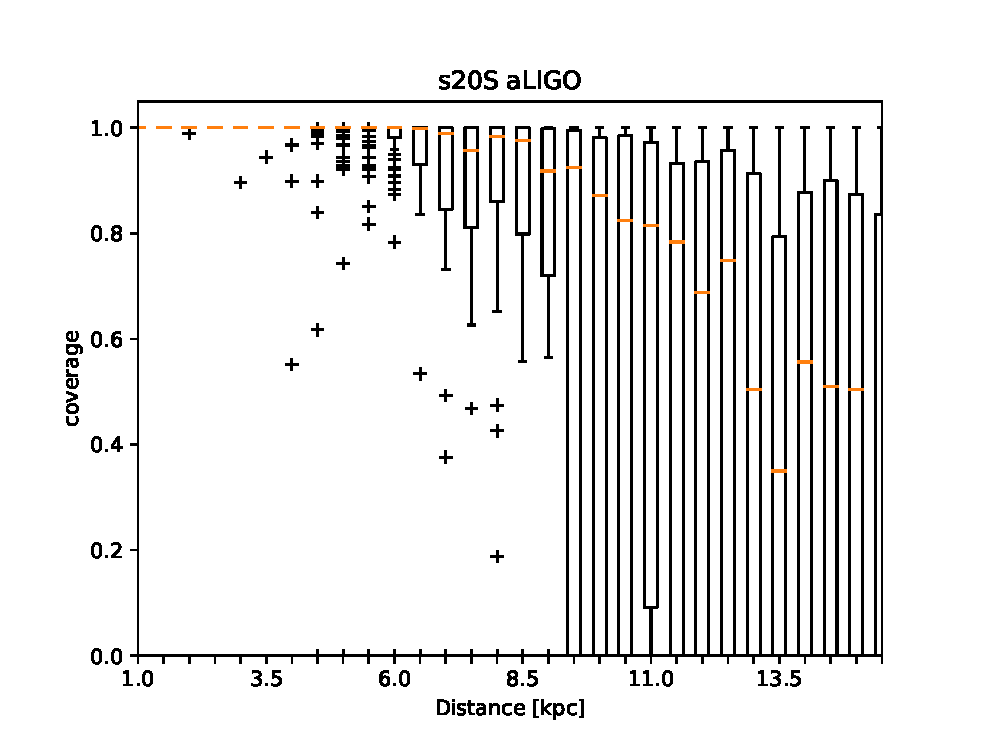
\includegraphics[width=0.5\textwidth]{plots/s20--SFHo_covpbb_boxplot_aLIGO} \\
    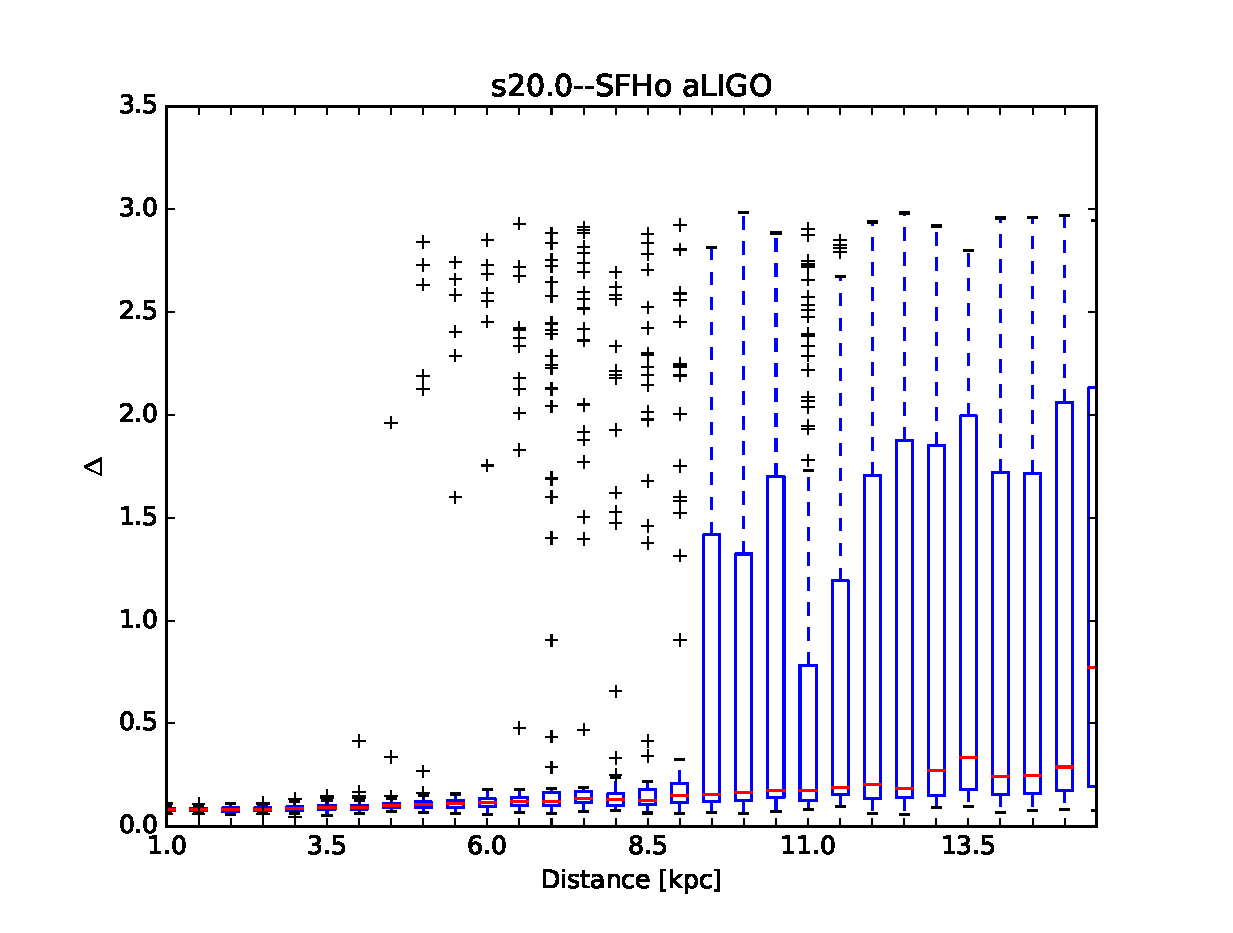
\includegraphics[width=0.5\textwidth]{plots/s20--SFHo_error_boxplot_aLIGO} \\
  \end{tabular}
    
 \caption{Boxplots of $coverage$ (upper panel) and $\Delta$ (lower panel) for {\texttt s20S} signal embedded in aLIGO noise at different distances from the Earth. 100 noise realisations is considered for each distance.}
  \label{fig:s20results}
\end{figure}

We have tested that the method does not depend on features of {\texttt s20S} using the 7
other waveforms of the {\it test set} described in section \ref{sec:simulations} covering
a large range of progenitor masses.

Figure \ref{fig:aLIGO_cov_allwvf} shows that apart {\tt s11.2--LS220} and to a lesser extent
{\tt s20.0--SFHo}, the ratio is well reconstructed for all waveforms up to $\sim$ 15kpc. In an
effort to better determine the maximal distance of the source at which we can reconstruct the ratio
we have run 100 simulations without injecting a signal and have measured $coverage$ for the
reconstructed ratios.
The median of $coverage$ as well as the 95 quartile are shown on Figure \ref{fig:aLIGO_cov_allwvf}.
The noise only median value is null in this case, but it can be different from zero because
the g-mode reconstruction algorithm is looking for a continuously frequency increasing track
in the spectrogram, starting between 0 and 200 Hz, where we expect the GW signal to be.
This is enhancing the probability of overlap. This effects explains why outliers can reach
values as high as 80\%.
Figure \ref{fig:aLIGO_prec_allwvf} shows $\Delta$ as function of the distance for the same signals
as well as the result when only noise is considered. 
In Table \ref{tab:results} we are reporting the distance $d_r$ at which $coverage$ median is lower
than 95\% of the noise only values. We have checked that $coverage$ and $\Delta$ provide similar
values.
These numbers are an estimate of the order of magnitude of the source maximal distance at which a
reconstruction of the ratio could be possible with current GW detectors.
They are also upper limits as we are taking into account the detector antenna response in our
simulation but consider the source is optimally oriented. 
Table \ref{tab:results} reports also $d_r$ for the advanced Virgo detector at design sensitivity.
Results are very similar to aLIGO, despite the detector sensitivity differences.
Note that Table \ref{tab:results} provides the distance at which one could detect a source
optimally oriented with a matched filter signal-to-noise ratio of 13.

\begin{figure}
  \centering
  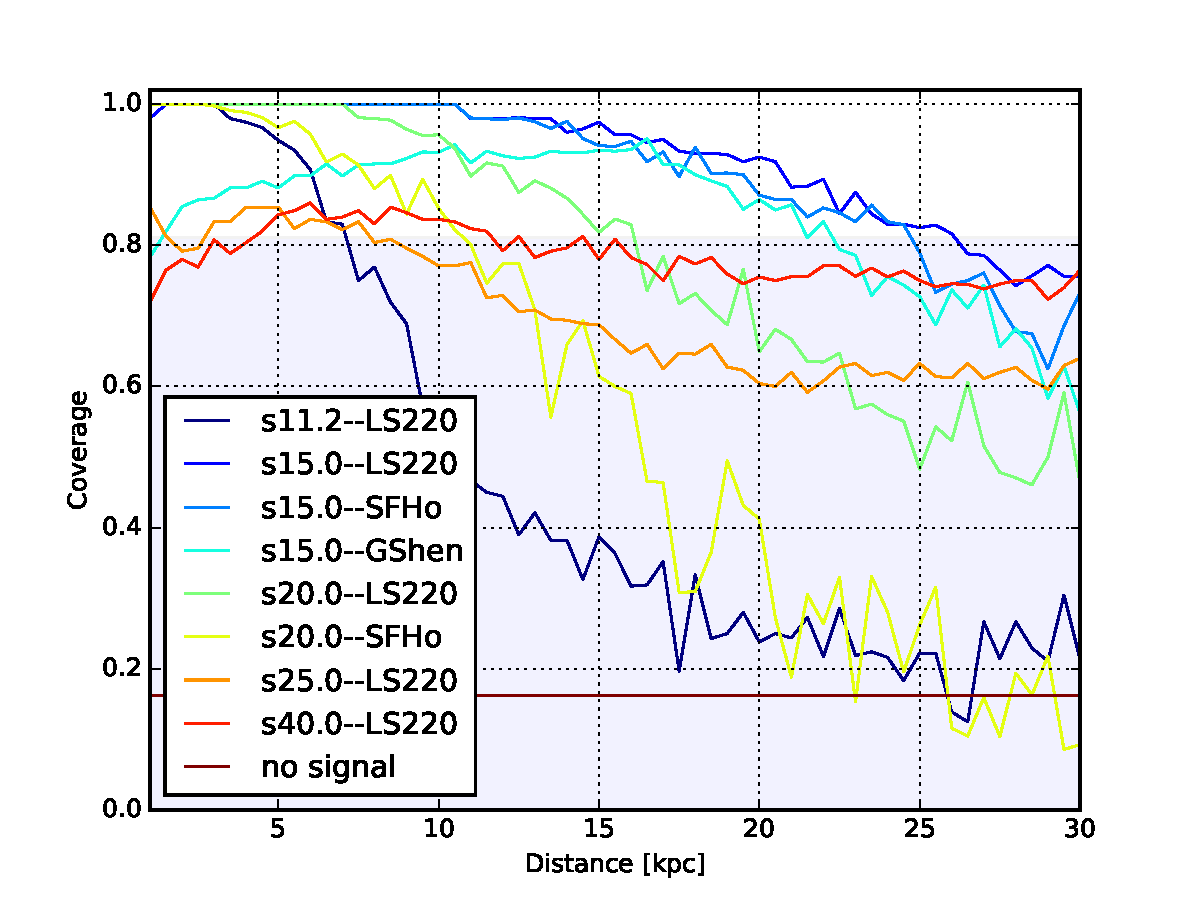
\includegraphics[width=0.5\textwidth]{plots/aLIGO_coverage_allwvfs}
 \caption{Median of $coverage$ for 8 CCSN waveforms embedded in aLIGO noise and located at different distance from the Earth. The ``no signal'' line and band show the median and first and third quartile of $coverage$ in absence of any signal.} \label{fig:aLIGO_cov_allwvf}
\end{figure}

\begin{figure}
  \centering
  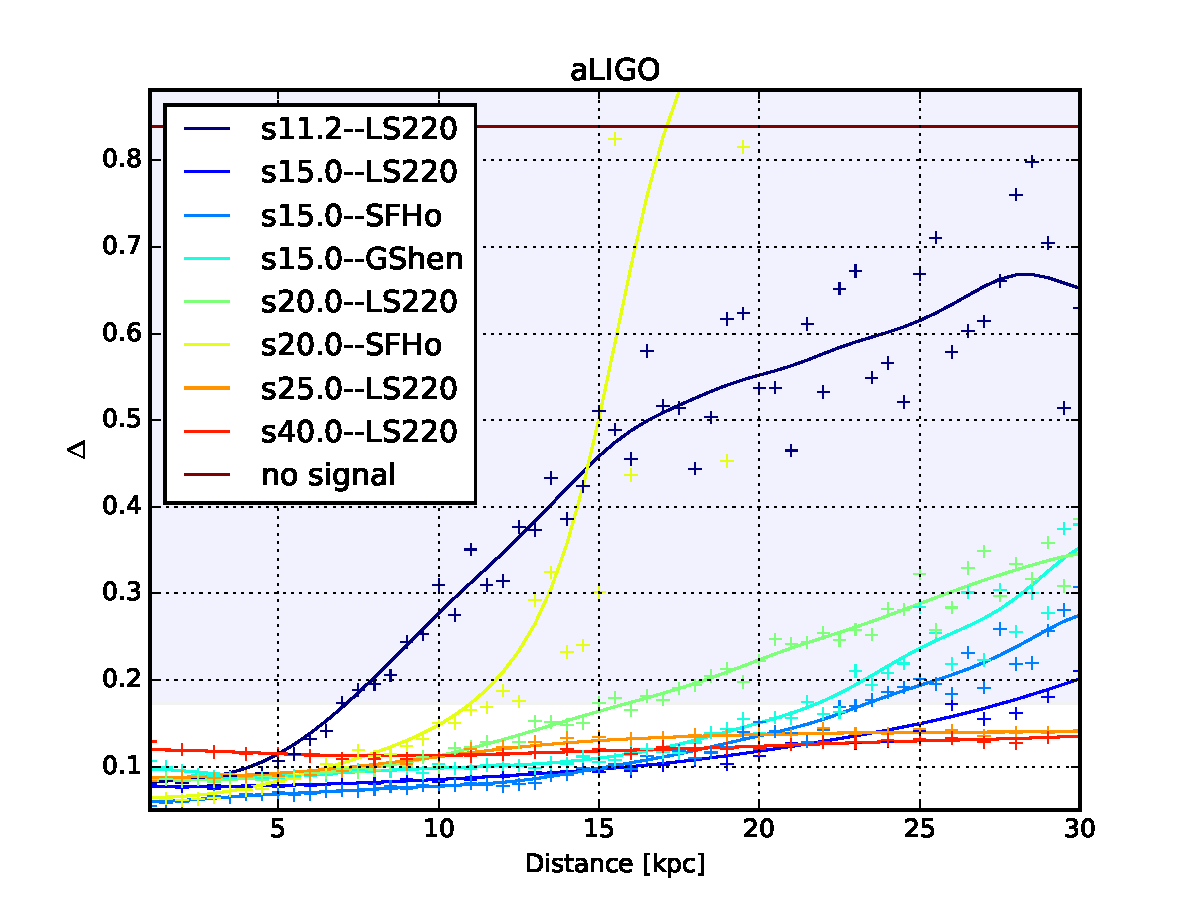
\includegraphics[width=0.5\textwidth]{plots/aLIGO_delta_allwvfs}
 \caption{Median of $Delta$ for 8 CCSN waveforms embedded in aLIGO noise and located at different distance from the Earth. The ``no signal'' line and band show the median and first and third quartile of $Delta$ in absence of any signal.} \label{fig:aLIGO_prec_allwvf}
\end{figure}

The same analysis has been performed using expected sensitivity curves for the third generation of
gravitational wave detectors. In Europe the Einstein Telescope project proposes to host in a 10-km
equilateral triangle configuration 3 low-power low-frequency cryogenic interferometers as well as 3
high-power high-frequency interferometers. Three sensitivity curves, ET-B, ET-C and ET-D corresponding
to different options and stages of the project~\cite{Hild_2011} are considered in this study.
The US based project Cosmic Explorer~\cite{reitze2019cosmic} is proposing to reach its design
sensitivity circa 2040 through two phases labeled CE1 and CE2 also shown in Figure~\ref{fig:spectrum}. 

Figure \ref{fig:s20--SFHo_all3G} shows $\Delta$ as function of the source distance for {\tt s20.0--SFHo}
waveform for the 5 3G detectors configurations. Overall, the ratio is well reconstructed up to distances
in the range \unit{100--200}[kpc] which represents an improved of at least a factor 10 with respect to
advanced LIGO and advanced Virgo detectors. We can also note that the Einstein Telescope results lay in
between the 2 Cosmic Explorer results. This is confirmed for all other waveforms, expect {\tt s25.0-LS220}
for which the maximal distance reach in CE2 is significantly lower than CE1. This is partly due to the
small variation of the reconstruction quality to the distance of the source making the estimation of $d_r$
rather incertain for this waveform. All results are summarized in Table \ref{tab:results} and Figure
\ref{fig:distances}. It is remarkable that with 3G detectors the ratio could be reconstructed for sources
located up to several hundred of kpc. It is nevertheless important to note the rather large range obtained
for the different waveforms probing a large range of progenitor masses.

\mab{add comment on the mass progenitor dependence}\\
\mab{say that the main depend is the SNR as shown by ddet}

\begin{figure}
  \centering
  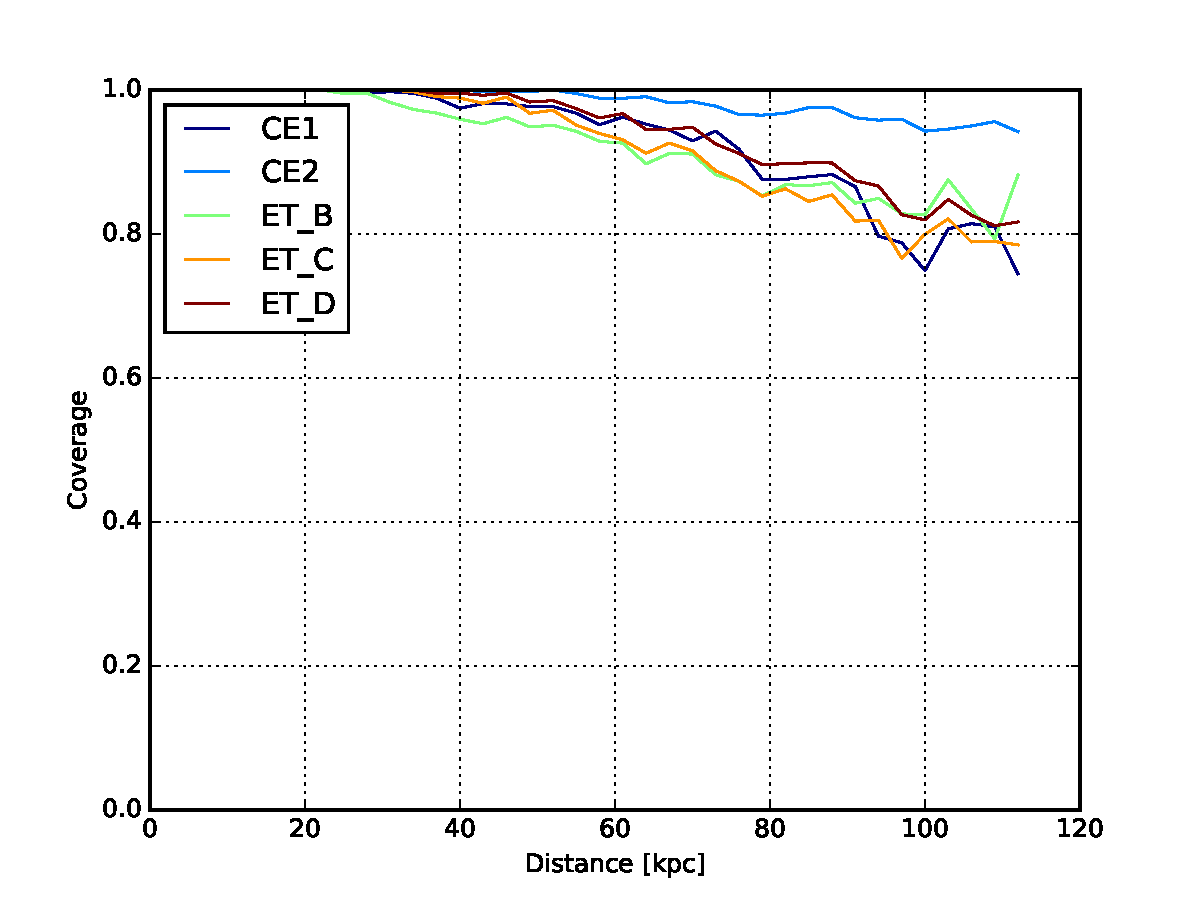
\includegraphics[width=0.5\textwidth]{plots/s20--SFHo_all3G}
  \caption{Median of $\Delta$ for s20.0--SFHo CCSN waveform embedded in 3G detectors noise and located at different distance from the Earth. } \label{fig:s20--SFHo_all3G}
\end{figure}

\begin{figure}
  \centering
  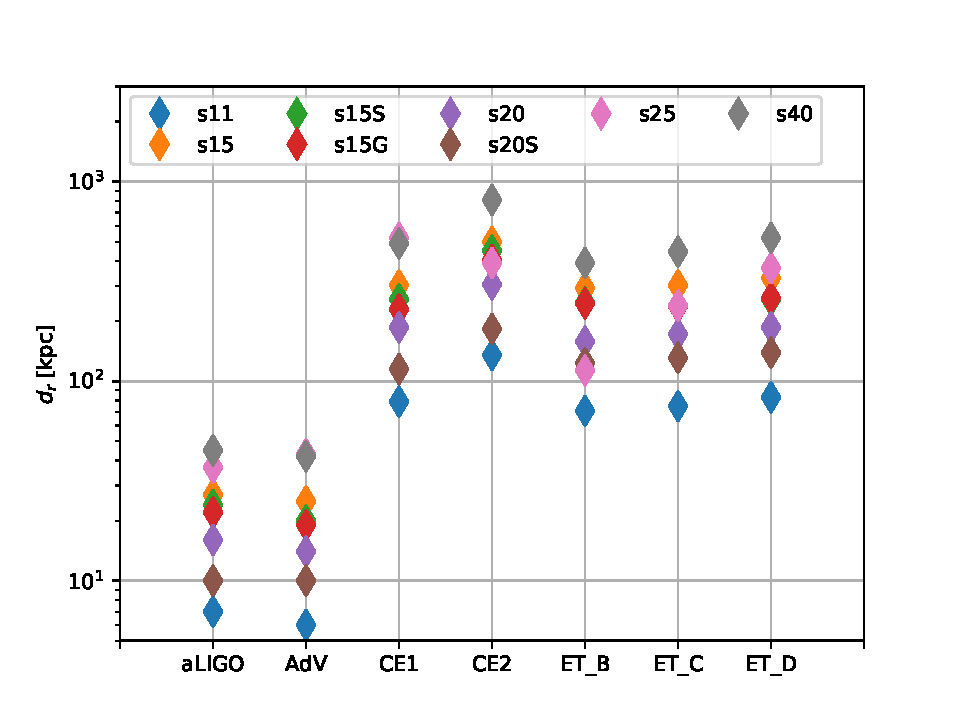
\includegraphics[width=0.5\textwidth]{plots/dist_allwvfs_2G3G}
  \caption{Maximal distance $d_{r}$ at which the ratio $r=M_{\rm PNS}/R_{\rm PNS}^2$ is reconstructed
    with good accuracy for a source optimally oriented with respect to the GW detectors for the 7 CCSN waveforms considered in this study.} \label{fig:distances}
\end{figure}



\begin{table}
  \centering
  \begin{tabular}{c|c|cccccccc}

\multicolumn{2}{c|}{}  & \texttt{s11} & \texttt{s15} & \texttt{s15S} & \texttt{s15G} & \texttt{s20} & \texttt{s20S} & \texttt{s25}  & \texttt{s40}\\   

\hline
\multirow{3}{*}{aLIGO} & $d_{r}$   & 7 & 28 & 24  & 22 & 16 & 11 & 38 & 46 \\
\cline{2-10}
                       & $d_{det}$ & 11 & 36 & 26 & 27 & 21 & 16 & 74 & 61\\
%                      & SNR      & 14 & 46 & 33 & 35 & 27 & 21 & 96 & 80\\

\hline
\hline
\multirow{3}{*}{ADV}   & $d_{r}$   & 7  & 26  & 20 & 19 & 15 & 10 & 43 & 42 \\
\cline{2-10}
                       & $d_{det}$ &  10 & 32 & 22 & 23 & 18 & 13 & 64 & 52\\
%                      & SNR      &  13 & 41 & 29 & 30 & 23 & 17 &  83 & 68\\

\hline
\hline
\multirow{2}{*}{CE1}   & $d_{r}$   & 79  & 304 & 258 & 229 & 187 & 115 & 524 & 490 \\
\cline{2-10}
                       & $d_{det}$ & 115 & 377 & 270 & 282 & 217 & 168 & 774  & 633\\
%                      & SNR      & 149 & 490 & 352 & 366 & 282 & 218 & 1006 & 822\\

\hline
\multirow{2}{*}{CE2}   & $d_{r}$  & 135 & 499 & 451 & 405 & 305 & 183 & 391 & 898 \\
\cline{2-10}
                       & $d_{det}$ & 197 & 649 & 468 & 489 & 375 & 294 & 1347  & 1100\\
%                      & SNR    & 256 & 843 & 608 & 635 & 487 & 382 & 1751 & 1430\\

\hline
\multirow{2}{*}{ET\_B} & $d_{r}$ & 71  & 293 & 248 & 245 & 158 & 123 & 113 & 392 \\
\cline{2-10}
                       & $d_{det}$ & 106 & 364 & 274 & 391 & 216 & 200 & 805 & 665\\
%                      & SNR      & 138 & 473 & 356 & 379 & 381 & 260 & 1046 & 865\\

\hline
\multirow{2}{*}{ET\_C} & $d_{r}$ & 75  & 302 & 239 & 237 & 172 & 131 & 239 & 446 \\
\cline{2-10}
                       & $d_{det}$ & 97 & 332 & 246 & 260 & 194 & 164 & 727  & 603\\
%                      & SNR      & 126 & 432 & 320 & 338 & 252 & 213 & 945 & 783\\

\hline
\multirow{2}{*}{ET\_D} & $d_{r}$ & 83  & 329 & 257 & 261 & 186 & 139 & 369 & 523 \\
\cline{2-10}
                       & $d_{det}$ & 107 & 368 & 271 & 285 & 213 & 174 & 796  & 661\\
%                      & SNR      & 140 & 477 & 352 & 371 & 277 & 227 & 1034 & 859 \\

  \end{tabular}
  \caption{%%
    Maximal distance $d_{r}$ at which the ratio $r=M_{\rm PNS}/R_{\rm PNS}^2$ is reconstructed
    with good accuracy for a source optimally oreinted with respect to the GW detectors
    considered in this study. $d_{det}$ is the distance at which one could detect a source
    optimally oriented with a matched filter signal-to-noise ratio of 13 in the  different
    GW detectors.
    %%
  }
  \label{tab:results}
\end{table}

